\textbf{COLUNI 2021 -- Questão 32}\par\medskip Observe e analise o mapa a seguir.

% COLUNI-AUTO-FIGURES-BEGIN
\begin{figure}[htbp]
\centering
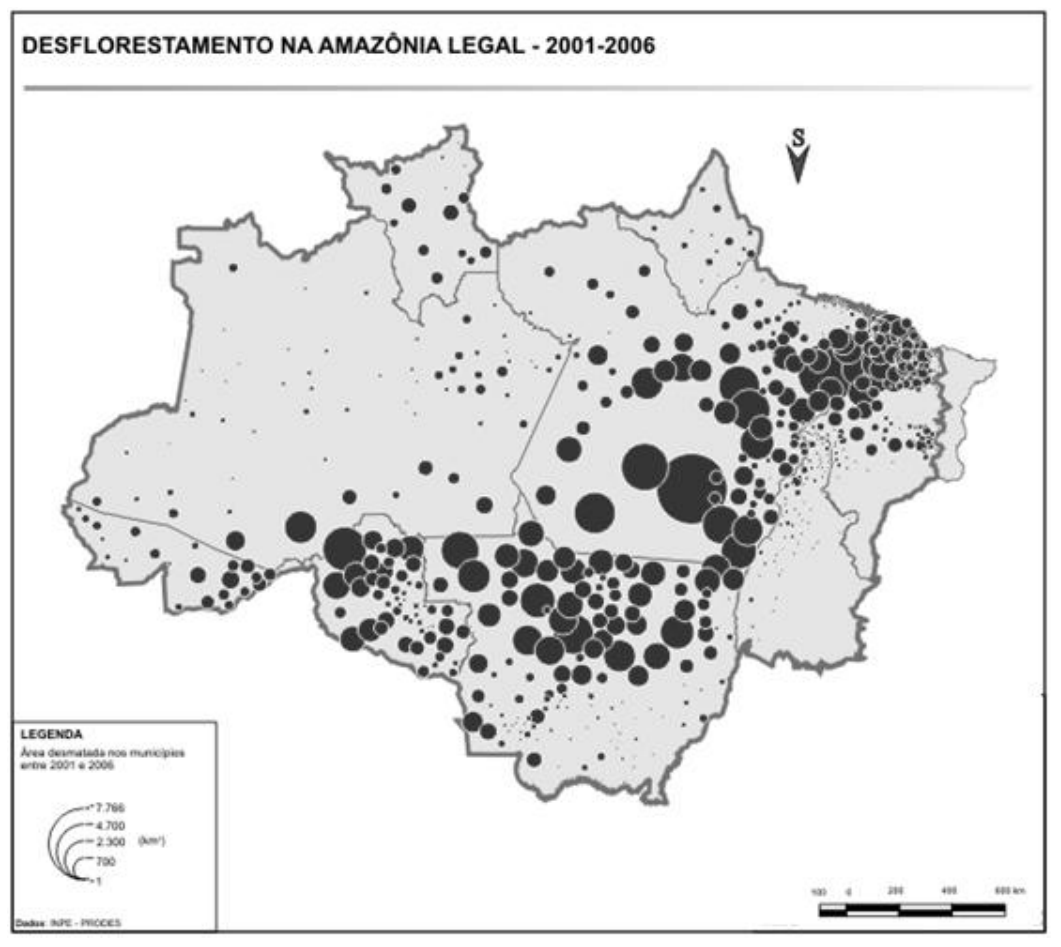
\includegraphics[width=0.95\linewidth]{static/simulados/coluni/figuras/2021/questao-32/figura-1.png}
\end{figure}
% COLUNI-AUTO-FIGURES-END

Disponível em: http://www2.fct.unesp.br/nera/atlas/configuracao\_territorial.htm. Acesso em: 22 nov. 2020.

\par

Com base no mapa e nos conhecimentos geográficos, é CORRETO afirmar que:

\begin{enumerate}
\item o mapa mostra apenas o desmatamento na região Norte e não inclui o Maranhão, pertencente à
      subregião Meio-Norte do nordeste brasileiro, com predominância de atividades extrativas.
\item o estado do Tocantins é o que apresenta maior taxa de desmatamento, fato associado ao intenso processo de
      urbanização ocorrido após 1988, como consequência do desmembramento com o estado de Goiás.
\item as áreas mais desmatadas estão localizadas nos estados de Rondônia, Mato Grosso, Pará e Maranhão,
      que representam espaços de intensos conflitos pela posse da terra e expansão da fronteira agrícola.
\item os estados do Acre, Roraima e Amapá, que possuem a menor densidade demográfica, são espaços
      ocupados apenas pela Floresta Amazônica e não possuem áreas de desmatamento.\end{enumerate}
